\documentclass[10pt,a4paper]{article}
\usepackage[margin=20mm,headheight=15pt]{geometry}
\usepackage{amsmath,amssymb,graphicx,booktabs,caption,enumitem,array,fancyhdr}
\usepackage{fontspec}
\usepackage[UTF8,fontset=windows]{ctex}

\setmainfont{Latin Modern Roman}
\usepackage[colorlinks=true,linkcolor=blue,urlcolor=blue,citecolor=blue]{hyperref}
\setlength{\parindent}{0pt}\setlength{\parskip}{5pt}
\setlist{nosep,leftmargin=1.5em,topsep=3pt}
\captionsetup{font=small,labelfont=bf,skip=4pt}
\pagestyle{fancy}\fancyhf{}\fancyhead[L]{ELEN90099 | LDI Preliminary Report}\fancyhead[R]{October 2026}\fancyfoot[C]{\thepage}
\setlength{\emergencystretch}{3em}
\begin{document}\begin{titlepage}\thispagestyle{empty}\centering\vspace*{22mm}
{\Large ELEN90099 Deep Learning\par}\vspace{8mm}
{\LARGE\bfseries 用电负荷与光伏出力的多步预测\\[4mm]初步实验、模型比较与验证计划\par}\vspace{10mm}
{\large Learn--Design--Implement Project\\Preliminary Report / 中文对照版\par}\vspace{12mm}
两位作者英文姓名与学号：待填写。\\[3mm]各节撰写责任：待填写。
\vspace{12mm}\begin{minipage}{0.88\textwidth}
\textbf{摘要。}本项目以原始 Monash 发布文件的固定16通道子集为对象，比较历史48小时到未来24小时的用电负荷和光伏出力预测。所有模型采用相同时间划分、训练区间标准化和评价起点；主实验使用三个固定种子、每次最多五轮训练，另进行单种子的历史窗口和训练数据量敏感性研究。模型覆盖持久化、日周期朴素基线、LSTM、GRU、卷积、CNN–LSTM、自写DLinear和简化PatchTST风格模型。初步结果显示，Electricity上patch模型具有进一步验证价值，而Solar上日周期基线更强。报告区分正式发布数据与本地合成信号、实测成本与部署推断，提供可复算预测、权重和SQLite实验记录，并明确终稿验证计划。
\end{minipage}\vfill
正文9页；封面和参考文献不计入初步报告正文页数。\\作者信息按当前约定保留待填写。
\end{titlepage}\setcounter{page}{1}
\section{引言、研究范围与相关工作}
\noindent\textit{本节撰写者：待填写。}


\subsection{工程问题与动机}
未来一天的用电负荷与光伏出力预测，可为调度和储能决策提供信息。本项目将目标限定为：仅凭过去48小时的目标观测，一次预测未来24小时，并比较增加模型复杂度能否带来值得其计算代价的误差改善。本项目研究监督式序列回归，不构建实际调度控制器，也不把预测误差直接换算为经济收益、电网安全改善或已部署效果。

研究采用Monash时序档案的Electricity小时级和Solar十分钟级两个独立任务\cite{monash,electricity,solar}。每个任务固定16条对齐序列，分别训练模型；不加入天气、日历、未来观测或跨数据集信息。这使信息条件更明确，同时限制模型预测突发天气变化的能力。Solar原始来源包含模拟数据；使用正式发布文件，不等于数据已成为真实电站部署记录\cite{solar}。
\subsection{研究问题与成功标准}
\begin{enumerate}
\item 在相同预测起点上，可训练模型是否优于持久化与日周期朴素基线？
\item 循环记忆、局部卷积、混合编码、线性分解和patch注意力，在误差和资源需求上有何差别？
\item 排名是否随预测距离、高负荷/活跃出力条件、历史长度和可用训练数据改变？
\end{enumerate}
评价采用原尺度MAE、RMSE、通道平均季节性MASE，以及实测训练和推理成本。超过较强的日周期基线，比只超过持久化更有说服力。只要协议明确、局限透明，复杂模型没有改善也可以构成有意义的初步结论。
\subsection{文献与课程知识的连接}
LSTM\cite{lstm}和GRU\cite{gru}通过门控更新状态；时间卷积用于检验局部滤波和权重共享；这些比较把递归计算、梯度学习和卷积机制落到同一预测任务。CNN–LSTM检验串联特征提取，但不预设其改善必然来自模块互补。DLinear\cite{dlinear}为复杂非线性与注意力是否必要提供反例参照；PatchTST\cite{patch}启发时间分块与跨通道共享编码，构成不同的时间表示。

当前模型均为自写PyTorch实现。注意力模型明确称为“PatchTST风格”：保留patch和通道独立思想，但不是原论文完整复现，也未直接导入Time-Series-Library。因此报告评价的是随附实现，不能把结果归为原论文官方排名。
\subsection{初步进度与终稿结构}
本次初步报告包含正式发布数据上的三种子主实验，以及单种子敏感性比较；可训练模型每次最多五轮。第2–5节给出数据、协议、设计和实现，第6–8节报告初步结果，第9节讨论局限、终稿任务和结论。终稿章节结构已完整呈现，未完成的进一步验证明确作为后续任务\cite{course}。两位作者与每节撰写责任按当前约定保留待填写，不沿用旧稿的虚构学号。

\clearpage
\section{数据来源核验与探索性分析}
\noindent\textit{本节撰写者：待填写。}


\subsection{发布文件与固定子集}
对下载ZIP和解压TSF保存SHA256；检查全部原始序列的有限性、共同长度/起点及训练区间非常数性。通过\texttt{series\_name}精确匹配通道，不将T5等名称当成数组索引。不插值、不额外转换单位；聚合发布版本的物理单位尚未独立确认，因此统一使用“原始发布单位”。
\begin{center}\small
\begin{tabular}{lrr}\toprule
属性 & Electricity & Solar\\\midrule
原序列数 / 使用数 & 321 / 16 & 137 / 16\\
每条长度 & 26,304 & 52,560\\
采样 / 日周期 & 1小时 / 24 & 10分钟 / 144\\
TSF起点 & 2012-01-01 00:00:01 & 2006-01-01 00:00:01\\
历史 / 预测步数 & 48 / 24 & 288 / 144\\
训练区间零值比例 & 0.0\% & 53.0\%\\
\bottomrule\end{tabular}\end{center}

选择仅使用前70\%区间：按均值稳定排序，分成四组，每组无放回抽四条；两个数据集分别重建seed42的NumPy随机数生成器。此次独立复现的选择与大纲固定名单一致。这覆盖不同平均水平，不证明子集代表总体。
\begin{quote}\small Electricity: T5, T8, T21, T30, T99, T133, T144, T146, T198, T219, T231, T251, T285, T291, T304, T309.\\Solar: T7, T9, T27, T28, T41, T58, T60, T64, T69, T77, T82, T97, T115, T123, T127, T131.\end{quote}
\begin{center}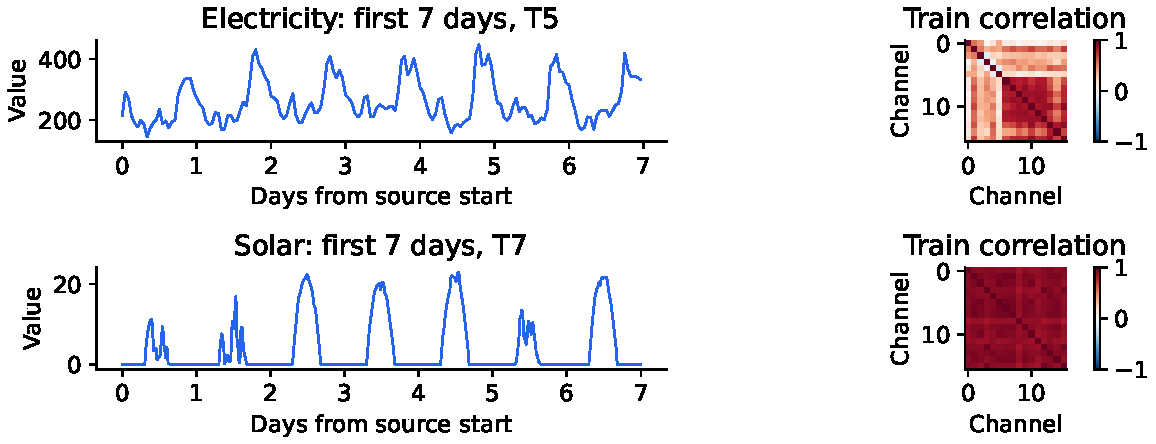
\includegraphics[width=\textwidth,height=6.1cm,keepaspectratio]{figures/data_overview.pdf}\captionof{figure}{固定首通道的前七天曲线与训练区间相关性；没有按预测好坏选择数据片段。}\end{center}
\subsection{对设计的启示与解释边界}
训练区间中的日内结构为日周期基线提供动机；相关性支持比较混合通道与独立通道模型，但不证明因果关系，也不能据此断言跨通道注意力必要。Solar大量零值可能压低总体误差，因此同时保留全时段和活跃出力条件指标。对象尺度不同，既需要逐通道标准化，也需要保留尺度归一化与原尺度两类评价。

两套数据分别来自不同年份和地区，不能拼接为对应负荷与电站。不擅自附加澳大利亚时区；发布文件中的共同起点和间隔仅支持格式对齐，不证明夏令时、当地时间或测量机制都经过验证。Solar的模拟来源还限制了结论向实际电站推广。

\clearpage
\section{预测问题定义与评价协议}
\noindent\textit{本节撰写者：待填写。}


\subsection{每个预测起点的信息边界}
设$X\in\mathbb R^{T\times C}$，$C=16$。起点$t$的输入是半开区间$X_{t-L:t}$，目标为$Y_t=X_{t:t+H}$。所有模型一次输出全部$H\times C$目标；Electricity的$(L,H)=(48,24)$，Solar为$(288,144)$。未来标签不进入历史输入。后续滚动起点可以使用此前已揭示的观测；这属于滚动起点评价，不是在测试区间开始时一次冻结整段信息。
\subsection{时间划分与标准化}
取$b_1=\lfloor0.70T\rfloor$、$b_2=\lfloor0.80T\rfloor$。训练、验证和测试目标分别完全位于$[0,b_1)$、$[b_1,b_2)$和$[b_2,T)$，目标窗口不能跨越其所属区间。历史上下文可来自更早分区，因为在预测时已经观测到。训练起点间隔3小时，验证与测试间隔1小时。只打乱已经隔离好的训练窗口，不随机划分重叠窗口。
\begin{center}\small
\begin{tabular}{lrrrrr}\toprule
数据集 & $b_1$ & $b_2$ & 训练窗口 & 验证窗口 & 测试窗口\\\midrule
Electricity & 18412 & 21043 & 6114 & 2608 & 5238\\
Solar & 36792 & 42048 & 2021 & 853 & 1729\\
\bottomrule\end{tabular}\end{center}

各通道仅以当前可用训练片段拟合$z_{tc}=(x_{tc}-\mu_c)/\max(\sigma_c,10^{-8})$；验证和测试使用相同统计量。预测反变换后才计算报告指标。训练与最佳权重选择使用标准化MSE，其通道权重和原尺度MAE不同，不能把训练损失排名直接等同于工程误差排名。
\subsection{指标与汇总方式}
设$N$个起点、预测跨度$H$、通道$C$，误差$e_{thc}=\hat y_{thc}-y_{thc}$，则
\begin{align}
\mathrm{MAE}&=\frac1{NHC}\sum_{t,h,c}|e_{thc}|,&\mathrm{RMSE}&=\sqrt{\frac1{NHC}\sum_{t,h,c}e_{thc}^2},\\
q_c&=\frac1{T_{\rm tr}-m}\sum_{s=m}^{T_{\rm tr}-1}|x_{sc}-x_{s-m,c}|,&\mathrm{MASE}&=\frac1C\sum_c\frac{\mathrm{MAE}_c}{\max(q_c,10^{-8})}.
\end{align}
其中$m$为一天，分母$q_c$仅使用该次训练区间\cite{mase}。整体RMSE不是通道RMSE的简单平均。MASE小于1表示优于训练区间的季节差分尺度，不自动意味着优于测试区间的日周期朴素预测。两套数据的MAE/RMSE单位及尺度不同，不能直接跨数据集比较数值大小。
\subsection{预测距离、条件切片与依赖性}
分别报告前4小时、完整24小时，以及按实际小时的逐距离误差。Electricity高负荷条件为真实值达到通道训练区间85\%分位数；Solar活跃条件为达到训练最大值的10\%。它们是事后评价条件，不是模型输入，也不是已确认的天文白天。主要结果保留所有原始负预测，不通过选择性截断改变成绩。

每小时滚动预测导致标签反复出现，窗口误差具有时间依赖。窗口数量不是独立样本数量；种子标准差仅描述训练随机性，因此不报告基于独立窗口假设的显著性结论。

\clearpage
\section{模型机制与设计理由}
\noindent\textit{本节撰写者：待填写。}


\subsection{无需训练的两个对照}
持久化令$\hat y_{t+h,c}=x_{t-1,c}$；日周期朴素预测令$\hat y_{t+h,c}=x_{t+h-m,c}$，其中$h=0,\ldots,H-1$且$H=m$。两者与神经网络接触相同历史，没有拟合参数，用于检验连续性与日内重复是否已解释大部分可预测变化。
\subsection{循环网络与卷积网络}
单层LSTM隐藏维64，利用门控记忆更新
\[
c_s=f_s\odot c_{s-1}+i_s\odot\tanh(W_g[x_s,h_{s-1}]+b_g),\qquad h_s=o_s\odot\tanh(c_s),
\]
其中$i_s,f_s,o_s$是sigmoid门\cite{lstm}。最后隐藏状态线性映射到$HC$个输出。门控提供可学习的记忆通路，但不保证五轮训练能学到周依赖。GRU通过更新门与重置门维护单隐藏状态\cite{gru}，减少循环参数。两者在每步混合16通道，并将整个历史压入末状态。

1D-CNN采用两层宽度3卷积，通道$16\to32\to64$，搭配BatchNorm与ReLU，自适应平均池化到16个位置，再由全连接层输出$HC$。池化前两层卷积的局部感受野为5步，池化汇总全历史的局部特征；这不是扩张TCN，也不证明它显式建模了远距离交互。对称padding仅在已观测历史内部运算，不泄漏未来目标。
\subsection{CNN–LSTM混合结构}
先用$16\to64$、宽度3卷积和BatchNorm/ReLU提取特征，再送入64维LSTM和直接预测头。设计假设是局部模式可简化循环编码。与LSTM比较属于架构比较，尚不能称为独立因果消融：输入表示和参数量也改变。容量匹配、移除前端等进一步控制留到终稿。
\subsection{线性分解与patch注意力}
DLinear以端点复制的25步移动平均得到趋势$T$和余项$R=X-T$，预测
\[\hat Y_{c,:}=W_TT_{c,:}+W_RR_{c,:}+b_T+b_R.\]
双分支映射在通道间共享，总参数$2H(L+1)$。余项不保证是纯物理季节分量。同样25步在Electricity覆盖25小时，在Solar仅4小时10分，因此相同步数不是相同物理滤波尺度\cite{dlinear}。

PatchTST风格模型逐通道分块，patch长度16、步幅8；映射到64维并加入可学习位置编码，经过两层Transformer（4头、前馈128、dropout0.1），展平后输出未来$H$步。注意力为$\mathrm{softmax}(QK^\top/\sqrt{d_k})V$\cite{patch}。通道折叠到batch维共享权重，不存在显式跨通道注意力。核心窗口的patch数量分别为5和35；patch物理长度为16小时与2小时40分，再次体现采样率影响。

当前自写实现采用PyTorch LayerNorm编码块、零初始化可学习位置向量和训练集整体标准化，没有RevIN；不能称为官方PatchTST精确复现。DLinear同样采用本地类的随机初始化。报告保留这些差别，不把本实现的观测推广为原模型所有实现的共同性质。

\clearpage
\section{实现、训练与可复现性}
\noindent\textit{本节撰写者：待填写。}


\subsection{初步预算与验证集选择}
初步配置预先固定为最多5轮、patience=3、batch=32、Adam学习率$10^{-3}$、weight decay=$10^{-4}$。主实验采用42、43、44三个种子，敏感性采用seed42；不依据测试排名进行特定模型搜索。这是明确受限的初步实验，不是收敛保证；终稿计划增加到最多20轮并通过验证集选择配置。

每轮遍历完整训练起点。验证MSE按所有目标元素累计后除以元素数量，避免末尾小batch获得过高权重。保留验证损失最低的状态，测试使用该状态而不一定是最后一轮。相同epoch上限并不等于参数、FLOPs、数据缩减时的optimizer steps或实际时间相同；这些量均记录。
\subsection{实测环境与资源}
新版运行设备为NVIDIA GeForce RTX 3060 Laptop GPU，PyTorch 2.5.1+cu121，Python 3.10.21，NumPy 2.2.6。
这是本地GPU结果，不是Colab T4实测。代码可在Colab运行，但应重新测量资源成本。

训练耗时包含训练轮次及验证，训练峰值采用CUDA allocated memory。推理为输入已驻留设备的模型前向，预热10次后同步计时30次；不含数据加载、传输、标准化和数据库/文件写入，不是端到端部署延迟保证。下表汇总主实验种子平均训练时间，以及各次推理中位数的平均；E/S分别代表Electricity/Solar。
\begin{center}\small
\begin{tabular}{lrrrr}\toprule
模型 & 参数 E & 参数 S & 训练秒 E / S & 中位毫秒 E / S\\\midrule
LSTM & 45,952 & 170,752 & 8.2 / 1.4 & 0.38 / 0.66\\
GRU & 40,704 & 165,504 & 3.4 / 1.3 & 0.41 / 0.50\\
1D-CNN & 401,568 & 2,369,568 & 4.3 / 1.7 & 0.72 / 0.77\\
CNN-LSTM & 61,504 & 186,304 & 4.5 / 1.7 & 0.98 / 1.00\\
DLinear & 2,352 & 83,232 & 3.0 / 1.2 & 0.52 / 0.52\\
PatchTST-style & 76,056 & 392,976 & 9.4 / 5.2 & 1.52 / 3.47\\
\bottomrule\end{tabular}\end{center}

\subsection{代码交付记录什么}
\texttt{prepare\_data.py}获取正式文件并保存哈希和ID；\texttt{data\_loader.py}验证数据来源及切分规则；\texttt{experiment.py}统一训练与评估。每次运行采用唯一目录，保存最佳权重、scaler、全部分区起点和完整测试预测。JSON与SQLite的\texttt{runs}表保留超参数、曲线、epoch、优化步数、环境、指标与相对路径。已实现数据库存储，但不宣称实现了向量检索。

\texttt{verify\_results.py --reload}从预测文件复算误差，检查源数据对齐、数据库一致性，并在CPU重载每个权重进行抽样预测对照。测试覆盖泄漏边界、来源缺失/篡改、指标、前后向梯度与通道策略。通过这些检查说明实现合同得到验证，不等于证明模型泛化。README提供获取数据、运行、重算、分析和编译步骤。

主结果均来自独立的新目录。旧稿的本地合成缓存、CPU数据库和标注不一致的T4图没有进入本报告；独立核验说明保留具体证据，避免把能够复算错误数据上的数字误当成正确的数据来源。

\clearpage
\section{初步结果与比较分析}
\noindent\textit{本节撰写者：待填写。}


下表为三个固定种子的均值$\pm$样本标准差。确定性基线的预测相同、种子标准差近零，三份记录不算三个独立预测试验。MAE/RMSE保留原发布尺度，MASE无量纲。表图直接由新版运行记录生成，不引用历史数据库成绩。
\subsection{Electricity：日周期是较强对照}
\begin{center}\small
\begin{tabular}{lrrr}\toprule
Model & MAE & RMSE & MASE\\\midrule
Persistence & 1,010.261 $\pm$ 0.000 & 3,091.327 $\pm$ 0.000 & 3.630 $\pm$ 0.000\\
Daily naive & 208.218 $\pm$ 0.000 & 732.211 $\pm$ 0.000 & 1.009 $\pm$ 0.000\\
LSTM & 262.727 $\pm$ 4.543 & 727.287 $\pm$ 15.818 & 1.310 $\pm$ 0.015\\
GRU & 262.592 $\pm$ 0.622 & 729.598 $\pm$ 2.779 & 1.304 $\pm$ 0.004\\
1D-CNN & 254.754 $\pm$ 1.493 & 696.794 $\pm$ 17.507 & 1.248 $\pm$ 0.026\\
CNN-LSTM & 267.183 $\pm$ 2.918 & 749.218 $\pm$ 9.099 & 1.310 $\pm$ 0.009\\
DLinear & 220.049 $\pm$ 0.504 & 665.572 $\pm$ 0.484 & 1.032 $\pm$ 0.003\\
PatchTST-style & 203.137 $\pm$ 3.301 & 636.246 $\pm$ 6.630 & 0.959 $\pm$ 0.012\\
\bottomrule\end{tabular}\end{center}
PatchTST风格模型的平均MASE为0.959，日周期基线为1.009，对应观测到的5.0\%下降。
该结果支持继续研究此子集上的patch时间编码，不代表普遍优势。原尺度MAE/RMSE受大通道影响更强，通道缩放MASE强调各通道相对误差，因此应同时阅读。循环和混合模型在五轮后的不足，可能来自优化不足、表示压缩或信息条件，不能证明这些架构不适用。
\subsection{Solar：先超过日周期基线，再讨论复杂度收益}
\begin{center}\small
\begin{tabular}{lrrr}\toprule
Model & MAE & RMSE & MASE\\\midrule
Persistence & 7.379 $\pm$ 0.000 & 12.546 $\pm$ 0.000 & 3.048 $\pm$ 0.000\\
Daily naive & 2.198 $\pm$ 0.000 & 5.712 $\pm$ 0.000 & 0.900 $\pm$ 0.000\\
LSTM & 3.653 $\pm$ 0.079 & 6.169 $\pm$ 0.192 & 1.493 $\pm$ 0.033\\
GRU & 3.665 $\pm$ 0.131 & 6.126 $\pm$ 0.175 & 1.498 $\pm$ 0.055\\
1D-CNN & 3.020 $\pm$ 0.045 & 4.888 $\pm$ 0.056 & 1.231 $\pm$ 0.018\\
CNN-LSTM & 3.462 $\pm$ 0.082 & 5.930 $\pm$ 0.146 & 1.414 $\pm$ 0.034\\
DLinear & 3.177 $\pm$ 0.037 & 5.236 $\pm$ 0.017 & 1.298 $\pm$ 0.015\\
PatchTST-style & 3.062 $\pm$ 0.036 & 5.100 $\pm$ 0.058 & 1.249 $\pm$ 0.015\\
\bottomrule\end{tabular}\end{center}
日周期基线平均MASE为0.900；PatchTST风格模型比它高38.9\%。
较强的日周期基线与重复出力形状一致，但不能据此证明云层可预测，也不能证明神经网络充分训练后无法改善。线性或注意力映射可能平滑尖峰，循环末状态还需输出较长的144步；当前没有天气变量来预判新云层变化。
\begin{center}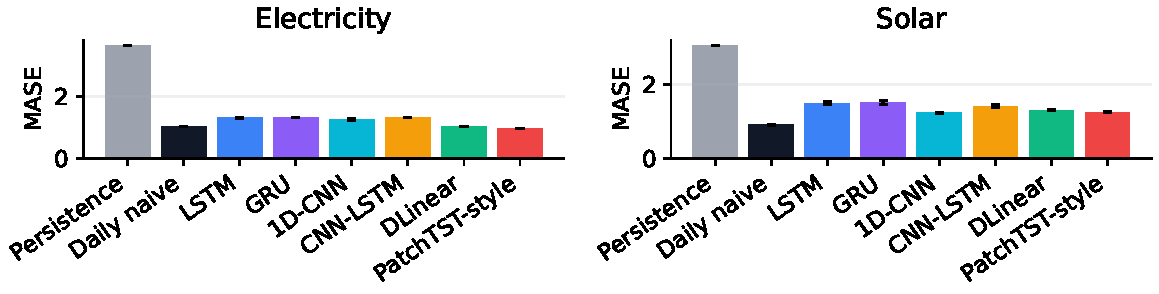
\includegraphics[width=\textwidth,height=3.7cm,keepaspectratio]{figures/comparison.pdf}\captionof{figure}{主实验初步比较；误差棒表示训练种子差异，不是独立测试日的置信区间。}\end{center}
\clearpage
\section{预测距离、条件误差与困难案例}
\noindent\textit{本节撰写者：待填写。}


\subsection{以实际小时解释预测距离}
\begin{center}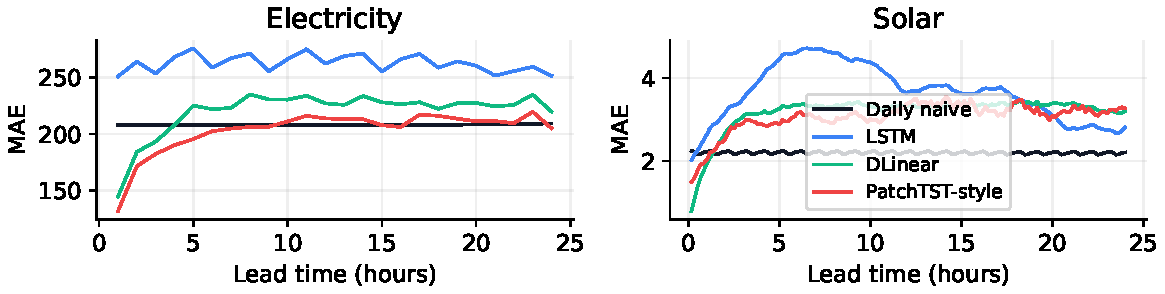
\includegraphics[width=\textwidth,height=3.9cm,keepaspectratio]{figures/lead_time.pdf}\captionof{figure}{三种子逐距离MAE（省略持久化）；横轴统一为小时。}\end{center}
所有模型均为直接多步输出，不把自身预测递归回灌。各输出与历史的关系、日内周期再次出现，都可能使误差非单调。持久化缺少未来相位对齐，日周期基线保留该相位。这些是本次滚动起点评价的现象，不能直接解释为递归误差累积。
\begin{center}\small
\begin{tabular}{lrrr}\toprule
数据集 & 模型 & 前4小时MAE & 条件MAE\\\midrule
Electricity & Daily naive & 208.122 & 401.885\\
 & LSTM & 259.245 & 461.200\\
 & DLinear & 182.470 & 409.421\\
 & PatchTST-style & 168.821 & 406.685\\
Solar & Daily naive & 2.202 & 5.655\\
 & LSTM & 3.112 & 5.256\\
 & DLinear & 2.463 & 4.896\\
 & PatchTST-style & 2.476 & 4.871\\
\bottomrule\end{tabular}\end{center}

条件列对应Electricity训练分位数定义的高负荷，或Solar训练最大值定义的活跃出力；同数据集/配置内各模型使用相同掩码。条件评价也改变通道和幅值构成，条件MAE较高本身不能证明特定物理失败机制。筛选比例保存在运行记录中。
\subsection{预先固定的困难场景规则}
\begin{center}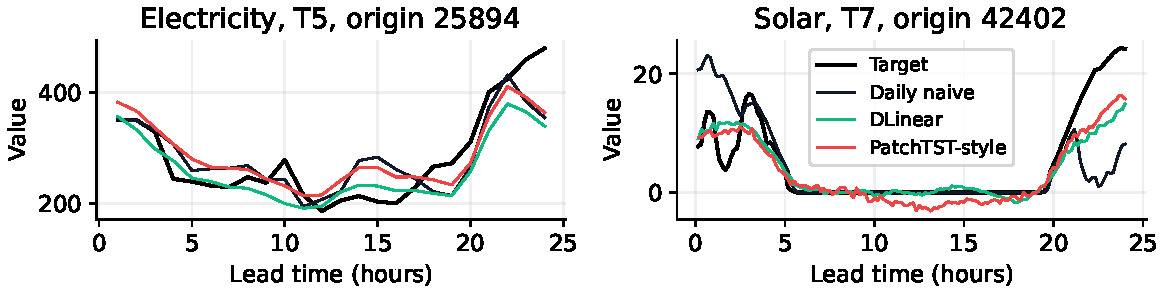
\includegraphics[width=\textwidth,height=3.6cm,keepaspectratio]{figures/hard_cases.pdf}\captionof{figure}{固定首通道，选择包含测试真实最大目标值的最早起点；不依模型误差选例，固定seed42而非最好种子。}\end{center}
这些峰值案例展示平均误差可能掩盖的幅值与相位偏差，但不是代表性或独立的总体证据。全部原始负预测仍计入主要分数；后续可另行比较所有模型统一非负截断的效果。\texttt{case\_selection.json}记录通道与源索引，能复现选择过程。

\clearpage
\section{历史长度与训练数据量敏感性}
\noindent\textit{本节撰写者：待填写。}


\subsection{受控实验设计}
LSTM和PatchTST风格模型均用seed42、最多5轮。历史取24/48/168小时：Electricity为24/48/168步，Solar为144/288/1008步。全部长度使用最大历史允许的共同训练起点，以及相同验证/测试起点。因此敏感性中的48小时运行是在较少的共同训练起点上重训，不能拿主实验成绩直接代替。

数据量实验保留原训练区间末尾25\%、50\%、100\%，结束时间固定$b_1$；输入与标签均位于保留片段内。各比例单独拟合可用训练scaler，固定通道和验证/测试区间不变，继续由验证损失选择最佳权重。100\%配置也重新运行，避免混入其他预算的结果。
\begin{center}\small
\begin{tabular}{lrrrrr}\toprule
数据集 & 因素 & 模型 & 小 & 中 & 大\\\midrule
Electricity & History & LSTM & 1.319 & 1.319 & 1.318\\
 &  & PatchTST-style & 1.019 & 0.965 & 0.841\\
 & Data & LSTM & 1.428 & 1.350 & 1.304\\
 &  & PatchTST-style & 0.968 & 0.977 & 0.946\\
Solar & History & LSTM & 1.550 & 1.489 & 1.499\\
 &  & PatchTST-style & 1.222 & 1.208 & 1.298\\
 & Data & LSTM & 2.692 & 2.636 & 1.531\\
 &  & PatchTST-style & 1.492 & 1.571 & 1.267\\
\bottomrule\end{tabular}\end{center}

\noindent\small History列为24/48/168小时；Data列为25/50/100\%；表内为季节性MASE。\normalsize
\begin{center}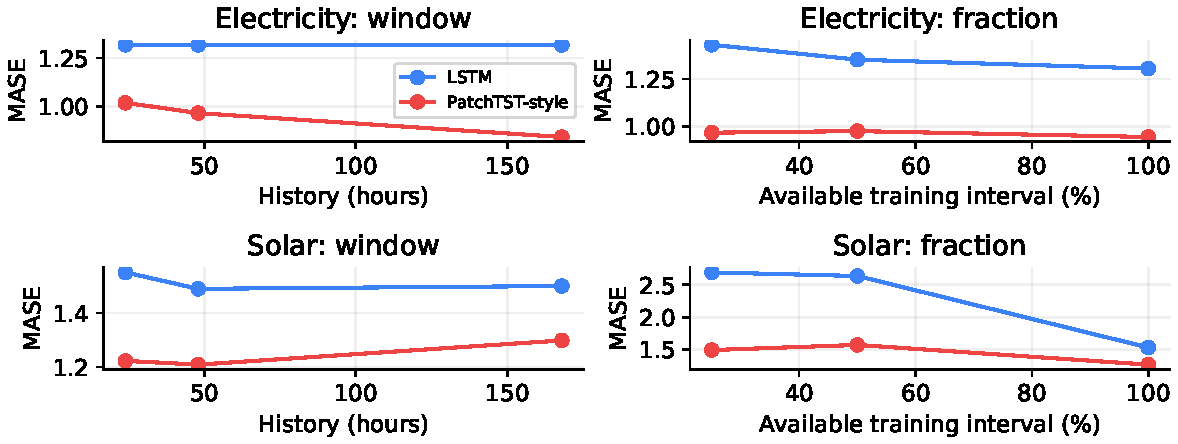
\includegraphics[width=\textwidth,height=5.7cm,keepaspectratio]{figures/sensitivity.pdf}\captionof{figure}{单种子受控敏感性；连接线仅连接已测配置，不表示插值性能或显著性。}\end{center}
\subsection{可以支持的解释与混杂因素}
Electricity 的 PatchTST-style 在该因素从最低到最高配置下，MASE 由 1.019 变为 0.841。Solar 的 LSTM 在该因素从最低到最高配置下，MASE 由 1.550 变为 1.499。Electricity 的 LSTM 在该因素从最低到最高配置下，MASE 由 1.428 变为 1.304。
端点差异不证明单调收益，仍需阅读中间配置。增加历史改变patch数量和输出头容量；即便循环模型参数量不变，计算量也改变。这是历史与容量共同变化的敏感性，不能作为纯记忆机制贡献证明。

缩减连续训练片段同时改变季节覆盖、数据新旧构成，以及五轮内的优化步数。各比例重新估计MASE分母，因此跨比例MASE变化还可能包含参照尺度变化；需结合JSON中的原尺度MAE/RMSE，不把所有差异归因于样本数量。多种子敏感性与固定更新步数控制留到终稿。

\clearpage
\section{工程判断、局限与终稿计划}
\noindent\textit{本节撰写者：待填写。}


\subsection{暂定工程选择}
应按任务比较精度与成本，而不是追求单个架构冠军。Electricity需要把patch模型的改善，与零参数日周期基线和轻量DLinear对照；Solar在当前信息与预算下，日周期基线是较强参照和可行的初始回退方案。复杂模型应通过高负荷或活跃出力等应用相关评价证明额外成本值得承担，当前误差变化没有直接转化为经济收益或控制效果。

参数量描述权重存储，峰值内存还包含激活与工作空间；两者都不能单独证明嵌入式可部署性。算子支持、数值精度、运行时与端到端延迟必须在目标设备检查。本地GPU测量不能推断T4吞吐或微控制器效果。任何帕累托判断都只对选定目标与测量条件有效，不是普遍最优。
\subsection{影响解释的局限}
\begin{enumerate}
\item 范围：固定16对象、单个时间区间不能证明其他用户、电站、年份或地区上的泛化。Solar有模拟来源，且天文和时区语义未独立验证。
\item 训练：五轮和通用设置属于初步预算，不意味着各架构已公平充分优化。三个种子只描述部分训练随机性，部分验证曲线到预算上限仍在改善。
\item 机制：容量、物理滤波跨度、归一化和输入表示都可能混杂架构比较；自写PatchTST风格并非完整原模型。当前不研究预训练基础模型、外生变量或跨数据集迁移。
\item 评价：窗口重叠使误差相关；MASE、原尺度指标和条件切片的权重不同。历史迭代曾查看测试区间，不能称为全新外部盲测。新版设置预先固定，未按测试排名调参或选种子。
\end{enumerate}
\subsection{终稿的具体完成路径}
\begin{enumerate}
\item 验证与预算：检查曲线，增加到最多20轮，并进行规模受限、可记录的验证集搜索；记录全部尝试，控制不同模型调参预算，不挑最好测试种子。
\item 敏感性与消融：各设置补多种子，同时报告MAE/RMSE与MASE；补固定更新步数控制、容量匹配的CNN前端比较，继续冻结通道与共同起点。
\item 误差分析：补逐通道结果；确认时间语义后再做工作日/周末；增加预定困难场景、残差依赖和统一截断比较。若需统计推断，应按时间块处理依赖，不能把窗口当独立样本。
\item 交付：确认姓名、学号与各节真实作者；终稿按另外的两人总计20页限制整理，并保留代码、数据库证据，准备课程口试和最多3分钟视频\cite{course}。
\end{enumerate}
\subsection{初步结论}
本次核验说明，基线强度和实验协议应先于模型复杂度。Electricity上的patch编码值得继续验证，Solar则暴露出当前预算下与日周期基线的明显差距。现阶段成果是可复现的初步比较、与实际实现一致的机制解释，以及检验这些观察能否在更充分训练和更广验证下成立的受控计划。
\clearpage
\begin{thebibliography}{9}\small
\bibitem{monash} R. Godahewa et al., ``Monash Time Series Forecasting Archive,'' NeurIPS Datasets and Benchmarks, 2021. \url{https://arxiv.org/abs/2105.06643}.
\bibitem{electricity} R. Godahewa et al., Electricity Dataset (Hourly Observations), Zenodo, record 4656140. \url{https://doi.org/10.5281/zenodo.4656140}.
\bibitem{solar} R. Godahewa et al., Solar Dataset (10 Minutes Observations), Zenodo, record 4656144. \url{https://doi.org/10.5281/zenodo.4656144}.
\bibitem{lstm} S. Hochreiter and J. Schmidhuber, ``Long Short-Term Memory,'' Neural Computation, 9(8), 1735--1780, 1997. \url{https://www.bioinf.jku.at/publications/older/2604.pdf}.
\bibitem{gru} K. Cho et al., ``Learning Phrase Representations using RNN Encoder-Decoder for Statistical Machine Translation,'' EMNLP, 2014. \url{https://arxiv.org/abs/1406.1078}.
\bibitem{dlinear} A. Zeng et al., ``Are Transformers Effective for Time Series Forecasting?'' AAAI, 2023. \url{https://arxiv.org/abs/2205.13504}.
\bibitem{patch} Y. Nie et al., ``A Time Series is Worth 64 Words: Long-term Forecasting with Transformers,'' ICLR, 2023. \url{https://arxiv.org/abs/2211.14730}.
\bibitem{mase} R. J. Hyndman and A. B. Koehler, ``Another Look at Measures of Forecast Accuracy,'' International Journal of Forecasting, 22(4), 679--688, 2006. \url{https://robjhyndman.com/papers/mase.pdf}.
\bibitem{course} ELEN90099 teaching team, LDI Project Manual v1, Project Options v1, Inspiration Project v1, and supplied Prelim Report instructions/rubric, 2026. Local course materials.
\end{thebibliography}
\end{document}